\section{Methodology}
\label{sec:method}

\begin{figure*}[t]
    \centering
    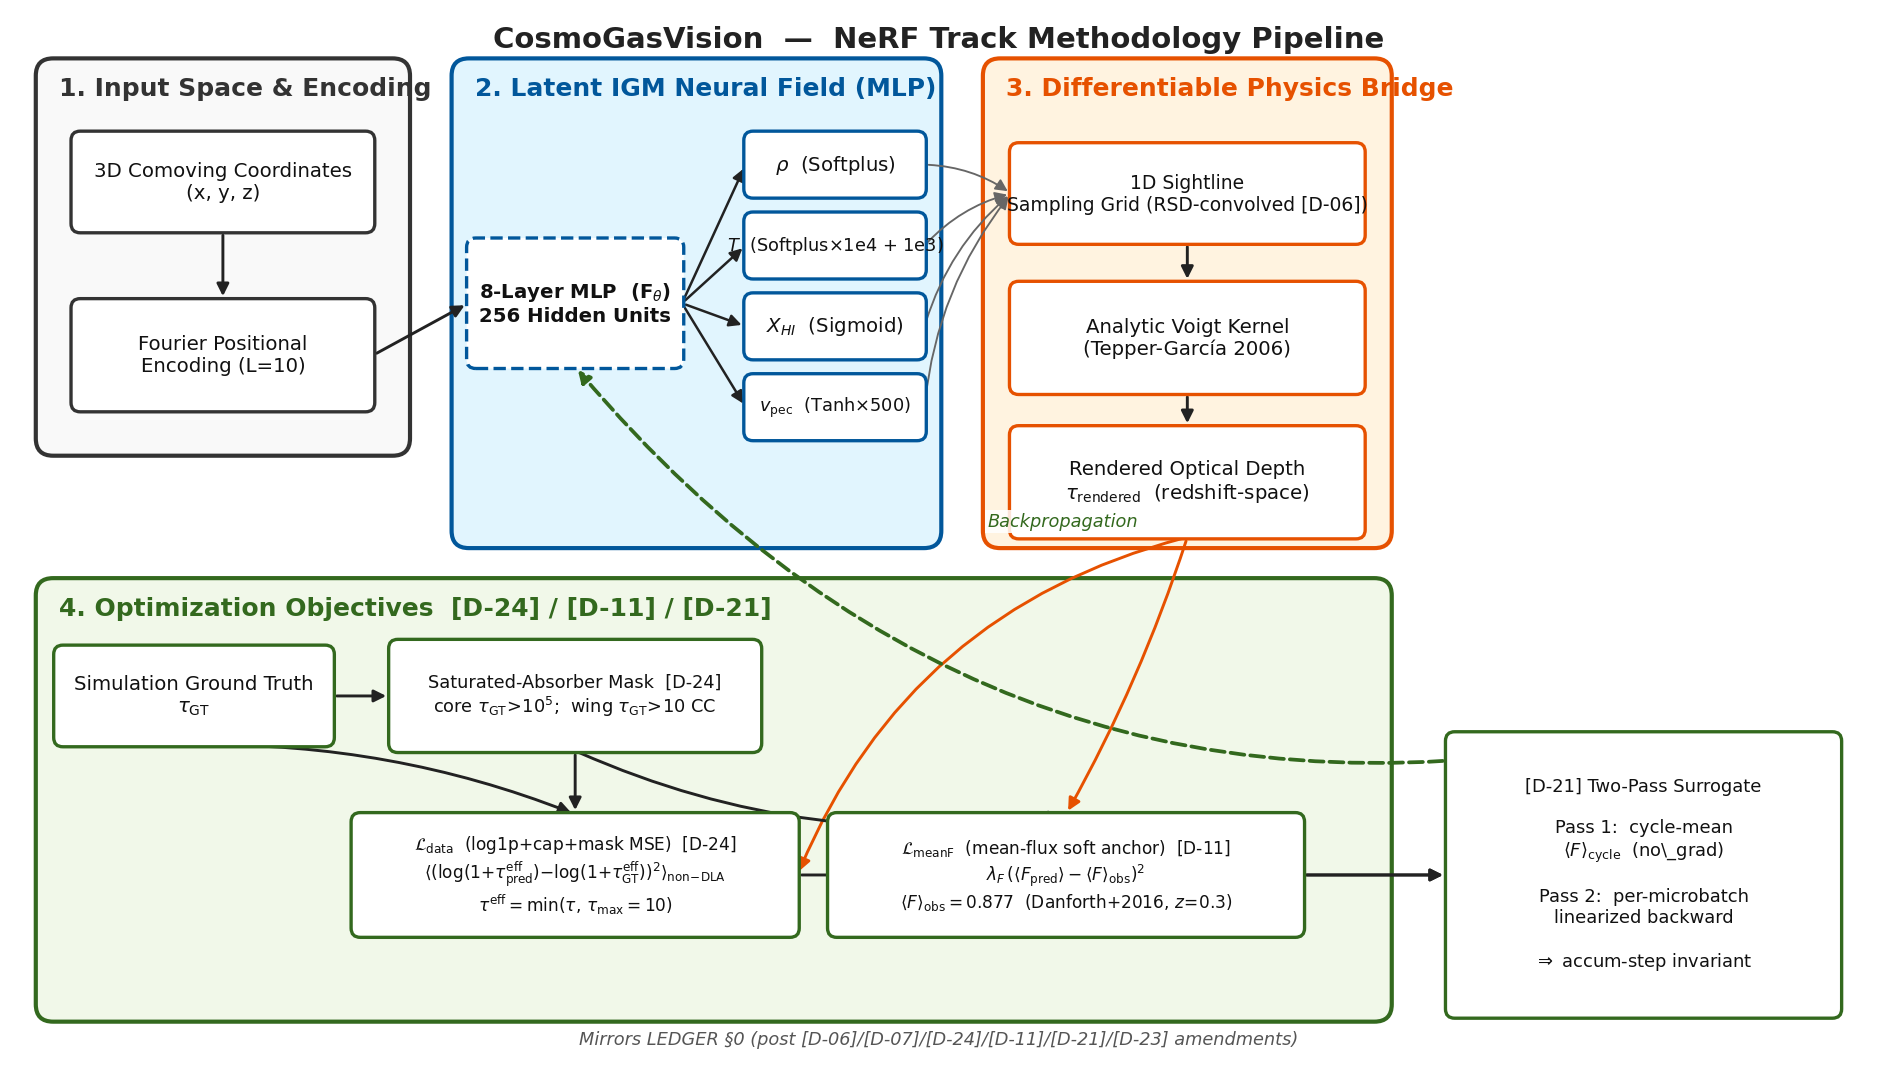
\includegraphics[width=\textwidth]{figures/method_pipeline}


    \caption{The IGM-NeRF tomography pipeline. An 8-layer / 256-unit MLP (494{,}084 trainable parameters) maps comoving 3D coordinates inside a 60 Mpc/h Sherwood box (normalized to $[0,1]^3$) through Fourier positional encoding ($L=10$) to four bounded astrophysical fields ($\rho/\bar\rho$, $T$, $X_{HI}$, $v_{\text{pec}}$); a differentiable RSD-convolved Voigt integrator with learnable amplitude $\mathcal{A}$ projects these fields to 1D optical depth $\tau(v)$, supervised against Sherwood ground truth under the [D-24] log1p+cap+mask loss with the [D-11]/[D-34] mean-flux anchor at $\langle F\rangle_{\text{obs}}(z=0.3) = 0.979 \pm 0.005$~\cite{kirkman2007}.}
    \label{fig:pipeline}
\end{figure*}

The core of \emph{CosmoGasVision} is an MLP $F_{\theta}: \mathbf{x} \to (\rho, T, X_{HI}, v_{\text{pec}})$, where $\mathbf{x} \in \mathbb{R}^3$ are comoving coordinates inside a 60 Mpc/h Sherwood box, normalized to the unit cube $[0, 1]^3$ by dividing by the simulation header field \texttt{box\_kpc\_h} = 60{,}000. The end-to-end pipeline --- coordinate normalization, Fourier positional encoding, bounded-output MLP, RSD-convolved Voigt projection, and log1p+cap+mask supervision with the mean-flux anchor --- is shown in Fig.~\ref{fig:pipeline}.

\subsection{Neural Field Architecture}
We adopt an 8-layer MLP with 256 hidden units per layer (494{,}084 trainable parameters). To resolve the small-scale filamentary structures of the Cosmic Web, we employ Fourier positional encoding~\cite{mildenhall2020nerf} for the input coordinates $\mathbf{x}$:
\begin{equation}
\gamma(\mathbf{x}) = (\sin(2^0\pi\mathbf{x}), \cos(2^0\pi\mathbf{x}), ..., \sin(2^{L-1}\pi\mathbf{x}), \cos(2^{L-1}\pi\mathbf{x}))
\end{equation}
where $L=10$ provides sufficient bandwidth for the spatial fluctuations in density and temperature; Lyman-alpha peak strengths spike nearly $100\times$ the mean overdensity in massive filaments, which sets a hard lower bound on $L$.

\subsection{Bounded Physics Layer}
To ensure the MLP outputs remain physically plausible, we apply field-specific activations in the final layer with explicit physical scales:
\begin{itemize}
    \item \textbf{Density} ($\rho/\bar{\rho}$): \texttt{Softplus}, unscaled. Overdensity is dimensionless and filament peaks reach $\sim 100$ in the linear regime of the activation.
    \item \textbf{Temperature} ($T$): $\texttt{Softplus}(x) \cdot 10^4 + 10^3$ K. The $10^3$ K floor matches the cold-IGM limit; the $10^4$ K scale anchors the typical warm IGM, with the WHIM tail at $10^5$--$10^7$ K reachable through the linear regime.
    \item \textbf{HI Fraction} ($X_{HI}$): \texttt{Sigmoid}, bounded to $[0, 1]$.
    \item \textbf{Peculiar Velocity} ($v_{\text{pec}}$): $\texttt{Tanh}(x) \cdot 500$ km/s. Defensible for the diffuse IGM at $z=0.3$ (typical $\pm 200$--$300$ km/s).
\end{itemize}

\subsection{Differentiable Physics Integrator}
The reconstruction is supervised by comparing rendered 1D optical depth $\tau_{\text{rendered}}(v)$ against the simulation ground-truth $\tau_{GT}(v)$ on the full velocity axis. We implement the optical depth as a redshift-space-distortion convolution that sums every source-bin's normalized line profile over every observed-velocity bin:
\begin{equation}
\tau(v_{\text{obs}}) = \mathcal{A} \sum_{\text{src}} n_{HI}^{\text{src}} \cdot \frac{H(a_{\text{src}}, x_{\text{src,obs}})}{b_{\text{src}}\sqrt{\pi}}
\end{equation}
where $x_{\text{src,obs}} = (v_{\text{obs}} - v_{\text{src}} - v_{\text{pec},\text{src}}) / b_{\text{src}}$, $b_{\text{src}}$ is the thermal Doppler parameter, and $\mathcal{A}$ is a learnable amplitude that absorbs the cross-section normalization $\sigma_0$, the comoving cell length $ds$, and the mean-column conversion $\bar{n}_H$ into a single scalar. The Voigt-Hjerting kernel $H(a, x)$ uses the Tepper-Garc\'ia~\cite{tepper2006voigt} analytic approximation:
\begin{equation}
H(a, x) \approx e^{-x^2} - \frac{a}{\sqrt{\pi} x^2} \big[ e^{-2x^2} (4x^4 + 7x^2 + 4 + 1.5x^{-2}) - 1.5x^{-2} - 1 \big]
\end{equation}
This allows the loss gradients to propagate back through the damping wings to the MLP parameters $\theta$.

\subsection{Lyman-alpha Forest Loss: Saturated-Absorber Mask, Cap, and Log-Space Supervision}
\label{sec:method:loss}
A naive per-bin MSE on raw $\tau$ is dominated by the rare saturated absorbers in the sightlines: damped Lyman-alpha systems (DLAs)~\cite{wolfe2005} and strong Lyman-limit systems~\cite{prochaska2010} produce line-center optical depths of $\tau_{\text{peak}} \sim 10^7$ in the Sherwood Physics-2/3/4 sightlines, four to five orders of magnitude above the diffuse forest. This saturation is forward-model-physical, not a label artifact, but it carries no usable structure information for tomography because $F = e^{-\tau}$ is numerically zero in those bins. We therefore replace the raw-$\tau$ supervision used in the Stage 2a smoke with \textbf{log-space supervision} (the methods contribution of this work, defended in Sec.~\ref{sec:method:loss:logspace}) plus two \textbf{defense-in-depth} safeguards --- a saturated-absorber detection mask and a forest cap --- retained against rare initialization-stress regimes (e.g., the Physics-2 tier-3 seed-0 softplus-saturation collapse documented in our cost-survey forensic, Sec.~\ref{sec:experiments:cost-survey-sweep}). An ablation on the Physics-1 tier-2 cost-survey configuration (Tab.~\ref{tab:s5s7-ablation}) shows that on this configuration the mask and cap are not load-bearing for convergence to the achieved loss floor; we report this null result as such and retain the safeguards for the stressed configurations on which the ablation was not exercised.

\textbf{Saturated-absorber detection.} Per-sightline, we flag bins with $\tau_{GT} > 10^5$ as saturated cores, then expand each core to its connected component of bins with $\tau_{GT} > 10$ (the saturated wing). The threshold $\tau_{\text{core}} = 10^5$ is derived from the Voigt line-center identity (Bolton \& Haehnelt~\cite{bolton_haehnelt2007} Eq. 5) for thermal Doppler broadening at $T = 10^4$ K:
\begin{equation}
\tau_0 \approx 5.2 \times 10^{-14} \cdot (T/10^4\,\text{K})^{-1/2} \cdot (N_{HI}/\text{cm}^{-2})
\end{equation}
which gives $\tau_0 > 10^5 \Leftrightarrow N_{HI} > 1.9 \times 10^{18}$ cm$^{-2}$. The threshold sits an order of magnitude below the canonical DLA boundary of $N_{HI} \geq 2 \times 10^{20}$ cm$^{-2}$~\cite{wolfe2005} and includes strong Lyman-limit systems at $N_{HI} \gtrsim 10^{17.2}$ cm$^{-2}$~\cite{prochaska2010}, so the mask is operationally conservative in the inclusion direction. Detection happens once per sightline at load time and is recorded as a per-bin sidecar mask carried through the loss reduction.

\textbf{Forest cap.} Surviving non-saturated bins are clipped at $\tau_{\max} = 10$ on both prediction and target before the loss is evaluated. The cap is calibrated on two grounds. First, the flux-PDF gate of Section~\ref{sec:experiments} evaluates KS distance on $F = e^{-\tau}$ over $F \in [0.05, 0.95]$, i.e., $\tau \in [0.051, 3.0]$; capping at $\tau_{\max} = 10$ ($F = e^{-10} \approx 4.5 \times 10^{-5}$) places the cap an order of magnitude above the science measurement range, so it does not bias the gate. Second, for strong-but-non-saturated absorbers ($\tau \in (3, 10]$), the cap bounds the gradient amplitude from the Lorentzian wing, where raw-$\tau$ MSE has non-Gaussian tail behavior that destabilizes optimization. The forest cap value $\tau_{\max} = 10$ is calibrated by the sensitivity gate of Sec.~\ref{sec:experiments:tau-max-sensitivity} (closed; $\tau_{\max} \in \{5, 10, 20\}$ vary observed $P_F(k_\parallel)$ by $\leq 0.02\%$).

\textbf{Log-space supervision.}
\label{sec:method:loss:logspace}
The data loss on the surviving bins is
\begin{equation}
\mathcal{L}_{\text{data}} = \big\langle \big( \log(1 + \tau_{\text{pred}}^{\text{eff}}) - \log(1 + \tau_{GT}^{\text{eff}}) \big)^2 \big\rangle_{\text{non-saturated}}
\label{eq:data-loss}
\end{equation}
where $\tau^{\text{eff}} = \min(\tau, \tau_{\max})$ and the average is taken over rays and over the unmasked velocity bins. The choice of $\log(1+\tau)$ as the supervision space is the methods contribution of this work, defended on physical grounds rather than as a citation of NN-supervision precedent. Lyman-alpha-forest opacity is approximately log-normally distributed in $\tau$ across the cool diffuse IGM~\cite{bi_davidsen1997, hui_gnedin1997} as a consequence of the Fluctuating Gunn-Peterson Approximation $\tau \propto \rho^{1.6} T^{-0.7}$ acting on a near-log-normal density PDF; supervising in $\log(1+\tau)$ matches this natural noise model. The $\log(1+\cdot)$ form additionally reduces to $\tau$ in the optically thin limit and is monotone with $-\log F$ for $\tau \gtrsim 1$, so the data loss and the mean-flux anchor (next subsection) pull on the network in compatible spaces. The mask and the cap are not part of this novelty claim; their role is the defense-in-depth one stated in the opening paragraph of Sec.~\ref{sec:method:loss}, and the four-cell ablation of Tab.~\ref{tab:s5s7-ablation} shows they are not load-bearing for convergence on the configuration we exercised.

\begin{table}[t]
    \centering
    \renewcommand{\arraystretch}{1.15}
    \setlength{\tabcolsep}{4pt}
    \begin{tabular}{l|cccc}
    metric & A: full & B: no-cap & C: no-mask & D: no-cap-no-mask \\
    \hline
    \texttt{loss}        & 0.0052      & 0.0052      & 0.0052      & 0.0052      \\
    \texttt{loss\_data}  & 0.0026      & 0.0026      & 0.0026      & 0.0026      \\
    \texttt{meanF} term  & $2.6203\!\times\!10^{-3}$ & $2.6205\!\times\!10^{-3}$ & $2.6201\!\times\!10^{-3}$ & $2.6203\!\times\!10^{-3}$ \\
    $\langle F\rangle$   & 0.9282      & 0.9282      & 0.9282      & 0.9282      \\
    \texttt{tau\_amp}    & 0.9983      & 1.0026      & 1.0003      & 1.0030      \\
    \end{tabular}
    \caption{\textbf{S5/S7 ablation on the [D-24] loss bundle.} Configuration: Physics-1 (``no feedback''), Tier-2 ($n_{\text{rays}}=256$), seed $=1$, 25k steps; broken anchor $\langle F\rangle_{\text{obs}}=0.877$ (apples-to-apples with the published P1-T2 baseline of Tab.~\ref{tab:batch2-t2-cost-survey}). All four cells converge to indistinguishable final states on \texttt{loss / loss\_data / meanF / $\langle F\rangle$} (four-decimal identity); only \texttt{tau\_amp} differs by $\leq 0.5\%$, in the calibration-degeneracy direction the [D-11] anchor sub-clause marks uninterpretable. \textbf{Verdict:} the cap and mask are not load-bearing for convergence on this configuration. They are retained as defense-in-depth against initialization-stress regimes (e.g., the Physics-2 tier-3 seed-0 softplus-saturation collapse documented in Sec.~\ref{sec:experiments:cost-survey-sweep}); their necessity on stressed configurations is \emph{not} tested by this ablation. \textbf{MLflow run\_ids:} \texttt{ca5a9ff1\dots} (full), \texttt{e563b72a\dots} (no-cap), \texttt{d691268c\dots} (no-mask), \texttt{fce098d3\dots} (no-cap-no-mask).}
    \label{tab:s5s7-ablation}
\end{table}

\begin{figure}[h]
    \centering
    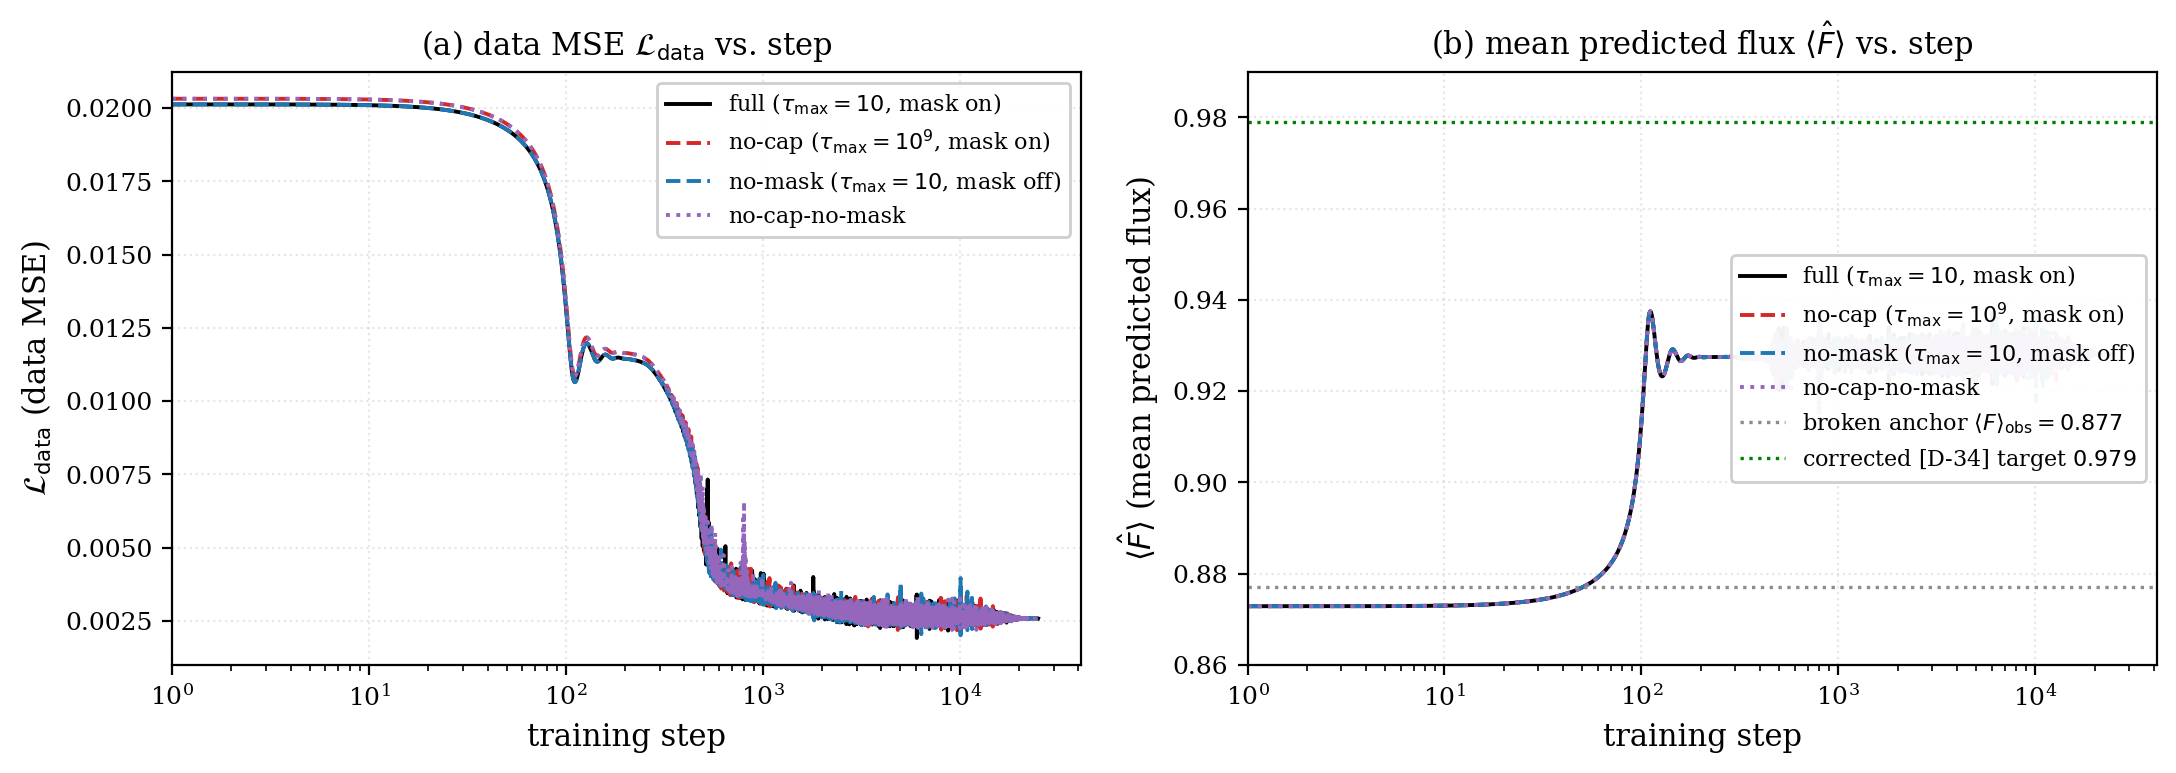
\includegraphics[width=\linewidth]{figures/s5s7_loss_curves.png}
    \caption{\textbf{S5/S7 ablation: training trajectories on T2-P1 seed=1, 25k steps, broken anchor $\langle F\rangle_{\text{obs}}=0.877$.} Left: data MSE $\mathcal{L}_{\text{data}}$ vs.\ step. Right: mean predicted flux $\langle\hat F\rangle$ vs.\ step (with the broken-anchor target 0.877 in gray and the corrected [D-34] target 0.979 in green; the model converges to $\langle\hat F\rangle\approx 0.9282$, between the two). All four cells converge to the same final regime ($\mathcal{L}_{\text{data}}=0.0026$, $\langle\hat F\rangle=0.9282$). The largest inter-cell divergence is at step~1: cells with the cap off (no-cap, no-cap-no-mask) start at $\mathcal{L}_{\text{data}}\approx 0.0203$ vs.\ $\approx 0.0201$ for cap-on cells, a $\sim 1\%$ relative gap that closes by step $\sim 100$ and is below line-width thereafter. \textbf{Verdict:} the cap and mask are not load-bearing on this configuration; they are retained as defense-in-depth (Sec.~\ref{sec:method:loss} opening; [D-38]).}
    \label{fig:s5s7-loss-curves}
\end{figure}

\subsection{Mean-Flux Anchor and Gradient Linearization}
The forward model is invariant under $\rho \to k\rho,\ \mathcal{A} \to \mathcal{A}/k$, so the data loss alone cannot fix the absolute amplitude of the recovered overdensity field. We break the degeneracy with the observational mean-flux constraint at $z = 0.3$:
\begin{equation}
\mathcal{L}_{\text{meanF}} = \lambda_F \big( \langle e^{-\tau_{\text{pred}}}\rangle - \langle F\rangle_{\text{obs}} \big)^2
\end{equation}
with verified value $\langle F\rangle_{\text{obs}}(z=0.3) = 0.979 \pm 0.005$ ($\tau_{\text{eff}} = 0.0212$) from the Kirkman et al.~\cite{kirkman2007} HST/FOS continuous-statistics Lyman-alpha-forest survey at $0 < z < 1.6$ (Table 2 + Section 4 power-law fit $D_A(z) = 0.016(1+z)^{1.01}$, evaluated at $z=0.3$), and $\lambda_F = 1.0$. The cost-survey runs reported in Sec.~\ref{sec:experiments:cost-survey-sweep} were trained against an earlier, broken anchor value $0.877$ (a $z\!\sim\!2$ value mislabeled as $z=0.3$ in project history); the [D-34] retraction explains why those runs are kept (anchor-invariance of the [D-13] structure gates) and which scalar reports are accordingly uninterpretable. The publication-class run trains against $0.979$. A $\pm 0.5\%$ uncertainty on $\langle F\rangle_{\text{obs}}$ propagates to a $\pm 0.5\%$ systematic on the absolute $\rho$ amplitude, but is invariant under the dimensionless structure metrics ($P_F$, $\xi_{\hat\rho,\rho}$, KS-distance on the flux PDF).

\textbf{Mask consistency.} The mean-flux reduction $\langle e^{-\tau_{\text{pred}}}\rangle$ and the data loss of Eq.~\ref{eq:data-loss} both apply the same saturated-absorber mask of Section~\ref{sec:method:loss}. This is load-bearing: a separately-derived prediction-side mask would be circular (saturation in $\tau_{\text{pred}}$ depends on the trainable parameters), so the per-sightline mask is taken from $\tau_{GT}$ at load time and reused unchanged in both reductions. The data loss and the anchor therefore see identical bin sets and the gradient identity below holds without correction terms for the masking operation.

\textbf{Two-pass linearization.} The mean-flux constraint is implemented as a two-pass surrogate to avoid \texttt{retain\_graph} in the microbatch grad-accumulation loop. Pass 1 runs the model under \texttt{torch.no\_grad()} to compute the cycle-mean predicted flux $F_{\text{cycle}}$ over all microbatches; Pass 2 then backpropagates a per-microbatch surrogate
\begin{equation*}
\mathcal{L}_{\text{mb}} = \mathcal{L}_{\text{data,mb}} + c \cdot \langle F\rangle_{\text{mb}}, \quad c = 2 \lambda_F (F_{\text{cycle}} - \langle F\rangle_{\text{obs}})
\end{equation*}
where $c$ is a constant for the cycle. By the chain rule $\partial \mathcal{L}_{\text{meanF}}/\partial \theta = c \cdot \partial F_{\text{cycle}}/\partial \theta$ and $\partial F_{\text{cycle}}/\partial \theta = (1/N_{\text{chunks}}) \sum_i \partial \langle F\rangle_{\text{mb},i}/\partial \theta$, so the surrogate's gradient is mathematically identical to the squared-loss gradient at the current parameter point. Re-linearization happens every optimizer step. Memory peak is one microbatch instead of \texttt{accum\_steps} microbatches.

\subsection{Training Configuration}
We optimize with AdamW ($\beta = (0.9, 0.999)$, weight decay $10^{-6}$), gradient L2-norm clipped at 1.0, on a single \texttt{ml.g5.xlarge} (NVIDIA A10G, 24 GB) SageMaker Training Job per tier. The cost-survey window adopts a tier-aware schedule, calibrated against the measured throughput of the Physics-1 tier-1 production run (0.119 s/step at chunk-size 64) rather than a uniform step count:

\begin{center}
\renewcommand{\arraystretch}{1.1}
\begin{tabular}{c|c|c|c|c}
Tier & $n_{\text{rays}}$ & $\mu$batch & accum. & max\_steps / warmup \\
\hline
T1 & 64    & 1024 & 1  & 50{,}000 / 1000 \\
T2 & 256   & 1024 & 1  & 25{,}000 / 1000 \\
T3 & 1024  & 256  & 4  & 12{,}500 / 500 \\
T4 & 16384 & 256  & 64 & 12{,}500 / 500 (deferred) \\
\end{tabular}
\end{center}

Microbatch values for tiers 3 and 4 are constrained by VRAM rather than convergence: the per-step chunk size is $\min(n_{\text{rays}}, \mu\text{batch})$, so chunk-size 256 saturates the linear-VRAM budget $\hat{V}_{\text{peak}} \approx 2.82 \cdot \min(n_{\text{rays}}, \mu\text{batch}) / 64$ GB derived from the tier-1 measurement (2.82 GB at 64 rays). The measured peaks (Tab.~\ref{tab:per-tier-vram}) sit $\geq 45\%$ under a 24 GB device VRAM budget across $\text{accum\_steps} \in \{1, 4, 64\}$.

\begin{table}[t]
    \centering
    \renewcommand{\arraystretch}{1.15}
    \begin{tabular}{c|c|c|c|c}
    Tier & $n_{\text{rays}}$ & chunk & accum & peak VRAM (GB) \\
    \hline
    T1 & 64    & 64  & 1  & 2.82  \\
    T2 & 256   & 256 & 1  & 11.20 \\
    T3 & 1024  & 256 & 4  & 11.23 \\
    T4 & 16384 & 256 & 64 & 11.77 \\
    \end{tabular}
    \caption{Stage 2b micro-grid per-tier peak VRAM measurements, validating the $\hat{V}_{\text{peak}} \approx 2.82 \cdot \min(n_{\text{rays}}, \mu\text{batch}) / 64$ GB scaling from [D-23]. All tiers fit $\geq 45\%$ under the 24 GB device VRAM budget; the linear model holds across the full $\text{accum\_steps} \in \{1, 4, 64\}$ range exercised by the production schedule.}
    \label{tab:per-tier-vram}
\end{table} The learning-rate schedule is per-tier linear warmup $0 \to 5 \times 10^{-4}$ followed by cosine decay $5 \times 10^{-4} \to 5 \times 10^{-6}$ over the remaining steps; checkpoints sync to S3 every 5{,}000 steps. Tier 4 is deferred to post-quota because its 64-chunk gradient accumulation makes its wallclock per cell dominate the survey budget; tiers 1--3 already span the survey-realistic sightline-density regime. Cost-survey runs are calibration evidence only; publication runs (post-quota) re-run the corresponding tier under the locked-in schedule.
